\documentclass[conference]{IEEEtran}
\IEEEoverridecommandlockouts
% The preceding line is only needed to identify funding in the first footnote. If that is unneeded, please comment it out.
\usepackage{cite}
\usepackage{amsmath,amssymb,amsfonts}
\usepackage{algorithmic}
\usepackage{graphicx}
\usepackage{textcomp}
\usepackage{xcolor}
\usepackage{hyperref}
\usepackage{booktabs}
\def\BibTeX{{\rm B\kern-.05em{\sc i\kern-.025em b}\kern-.08em
    T\kern-.1667em\lower.7ex\hbox{E}\kern-.125emX}}

\begin{document}

\title{TerraTrust: Geospatial Credit Intelligence for Rural Banking}

\author{\IEEEauthorblockN{Shreedhar K B (23BCS126)\thanks{\textbf{Project Source Code \& Datasets available at: \textcolor{blue}{\url{https://github.com/shreedharkb/TerraTrust}}}}}
\IEEEauthorblockA{\textit{Indian Institute of Information Technology, Dharwad}\\
Dharwad, Karnataka, India \\
23bcs126@iiitdwd.ac.in}
}

\maketitle

\begin{abstract}
Access to fair agricultural credit in rural India is fundamentally hampered by the absence of formal financial histories, verifiable land productivity data, and localized environmental risk assessments. Traditional banking models rely heavily on static paper trails and heuristic credit scoring, a system that structurally disadvantages smallholder farmers and simultaneously exposes lenders to uncalculated systemic risks. This paper introduces TerraTrust, an end-to-end Geospatial Intelligence Platform designed to mitigate these challenges. TerraTrust replaces arbitrary heuristic credit scoring with a purely data-driven, machine-learning-backed approach. By aggregating live multispectral satellite imagery and correlating it with global soil and climate datasets, the platform generates a verifiable, bias-free Visual Credit Score for geographic regions, specifically targeting Taluks in Karnataka. This research details the architecture, machine learning framework, and Explainable AI (XAI) components of TerraTrust, demonstrating a highly scalable solution capable of evaluating credit risk with sub-second inference latency. Extensive evaluation reveals that the stacked hierarchical modeling approach effectively isolates environmental variables from socioeconomic factors, significantly improving the fairness and accuracy of loan disbursement decisions.
\end{abstract}

\begin{IEEEkeywords}
Geospatial Intelligence, Rural Banking, Machine Learning, Explainable AI, Satellite Imagery, Credit Scoring, Precision Agriculture
\end{IEEEkeywords}

\section{\textbf{Introduction}}
The agricultural sector forms the backbone of the Indian economy, employing a vast majority of the rural population and contributing significantly to the national Gross Domestic Product (GDP). Despite its critical importance, financial inclusion for smallholder farmers remains a persistent challenge. Access to formal credit is often the primary bottleneck restricting agricultural growth, technological adoption, and ultimately, farmer prosperity. 

Traditional financial institutions depend predominantly on historical financial records, collateral verification, and credit scores derived from formal banking activities. Unfortunately, these conventional metrics are intrinsically biased against rural demographics, where transactions are frequently informal, and verifiable land ownership data is scarce or disputed. This reliance on static, often outdated paper trails leads to two significant, compounding issues. 

Firstly, it results in the widespread financial exclusion of millions of capable, productive farmers who lack the requisite documentation to prove their creditworthiness to institutional lenders. Secondly, it forces lending institutions to fall back on arbitrary heuristic risk assessments, which fail to capture the dynamic and hyper-local environmental realities that dictate agricultural success. The inability to accurately quantify agricultural risk exposes lenders to systemic defaults, especially in the face of increasingly erratic climate patterns and extreme weather events brought on by global climate change.

To bridge this gap, there is an urgent need for an objective, data-driven approach to agricultural credit scoring that bypasses the limitations of traditional financial history. This paper presents \textit{TerraTrust}, a comprehensive Geospatial Intelligence Platform designed to revolutionize rural banking. TerraTrust leverages the proliferation of high-resolution, high-frequency satellite imagery and global environmental datasets to construct a holistic profile of agricultural potential and environmental risk at the hyper-local level.

By utilizing advanced machine learning techniques, TerraTrust processes vast quantities of multispectral data to assess crop health, soil quality, and water availability. This environmental intelligence is then synthesized to produce a verifiable, bias-free \textit{Visual Credit Score}. The system is specifically calibrated and evaluated for various regions (Taluks) within the state of Karnataka, India, serving as a robust proof-of-concept for a globally scalable solution.


\begin{figure*}[htbp]
\centerline{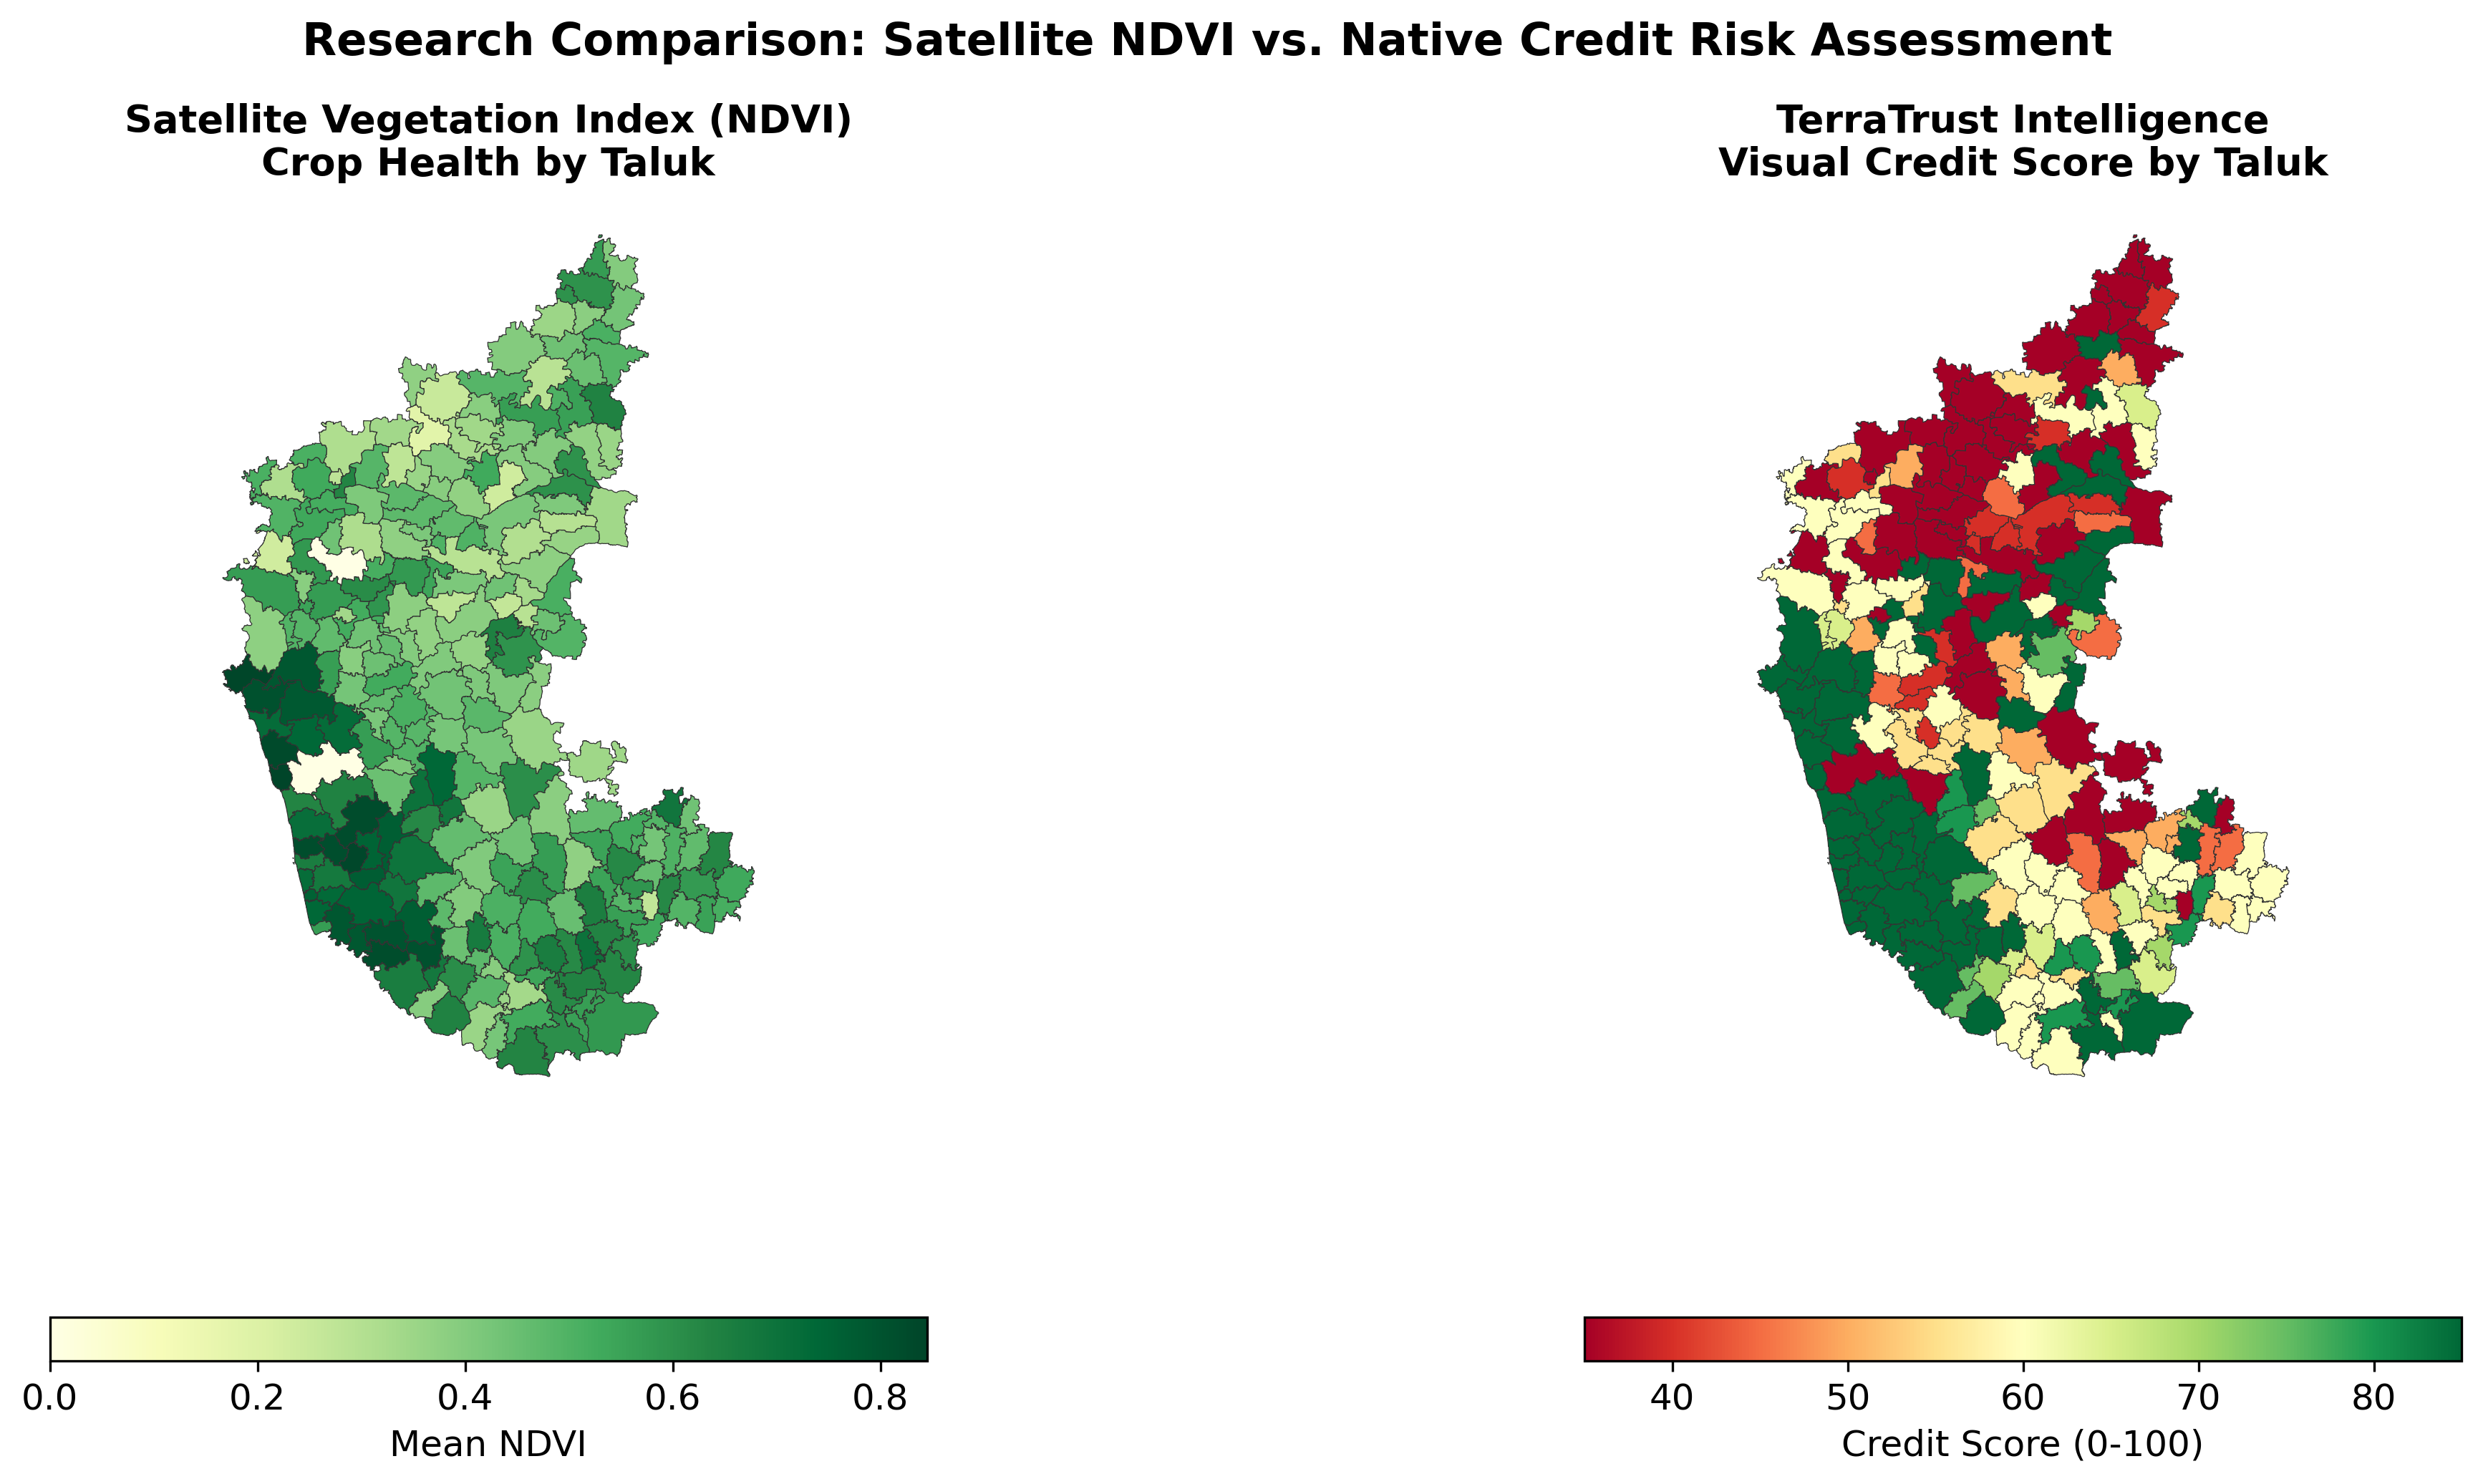
\includegraphics[width=\linewidth]{results_and_visualizations/Comparison_Maps/Comparison_NDVI_vs_Credit.png}}
\caption{Dual Choropleth Comparison: Satellite Vegetation Index (Annual Mean NDVI) versus the Machine-Learning-derived Visual Credit Score across Karnataka, showcasing the final output of the intelligence dashboard.}
\label{fig:ndvi_credit}
\end{figure*}

\section{\textbf{Background and Related Work}}
The intersection of satellite remote sensing, artificial intelligence, and financial technology (FinTech) has garnered significant attention in recent years. Early efforts in agricultural risk assessment primarily relied on macro-economic data and coarse-resolution weather models. However, the advent of open-access, high-resolution satellite constellations like the European Space Agency's Copernicus program (Sentinel series) and NASA's Landsat program has catalyzed a shift towards precision agriculture and hyper-local risk modeling.

Burke and Lobell \cite{b1} demonstrated the efficacy of using satellite imagery to assess crop yield variations in smallholder African systems, proving that remote sensing can act as a reliable proxy for economic output. Similarly, Dong et al. \cite{b2} utilized multi-temporal Landsat imagery to map agricultural practices, highlighting the potential of time-series analysis in understanding land use dynamics.

In the realm of credit scoring, there has been a push to move beyond traditional FICO-style models. However, most alternative credit scoring models focus on digital footprints (e.g., mobile phone usage, utility payments) rather than physical environmental factors. TerraTrust differentiates itself by establishing a direct causal link between the biophysical parameters of a region (soil health, water stress, vegetation vigor) and the systemic risk associated with lending in that region.

Furthermore, the deployment of machine learning in high-stakes domains like finance necessitates transparency. Lundberg and Lee's \cite{b4} introduction of SHAP (SHapley Additive exPlanations) provided a robust theoretical framework for interpreting complex models. TerraTrust heavily integrates SHAP to ensure that the generated credit scores are not only accurate but legally defensible and logically sound to agronomists and loan officers alike.

\section{\textbf{System Architecture}}
The TerraTrust platform is engineered as a modern, scalable data science pipeline, seamlessly integrating specialized geospatial libraries with a robust machine learning backend. The architecture is designed for low-latency inference, enabling real-time risk assessment for loan officers via an interactive spatial dashboard.

\subsection{\textbf{Technology Stack}}
The core logic of TerraTrust is implemented in Python 3.10+, leveraging fundamental data science libraries such as \texttt{pandas} and \texttt{numpy} for high-performance vectorized operations. For geospatial manipulation, the system utilizes \texttt{geopandas}, \texttt{shapely}, and \texttt{pyproj}, allowing for efficient processing of vector geometries (e.g., Taluk boundaries). Raster data processing is handled primarily by \texttt{rasterio}.

The machine learning framework relies heavily on \texttt{xgboost} \cite{b3} and \texttt{scikit-learn}, chosen for their superior performance with tabular geospatial features and their inherent compatibility with tree-based explainability tools. The frontend is powered by Streamlit, providing a premium, interactive web interface enhanced with custom HTML/CSS and \texttt{folium} for dynamic map visualizations. 

\begin{figure*}[htbp]
\centerline{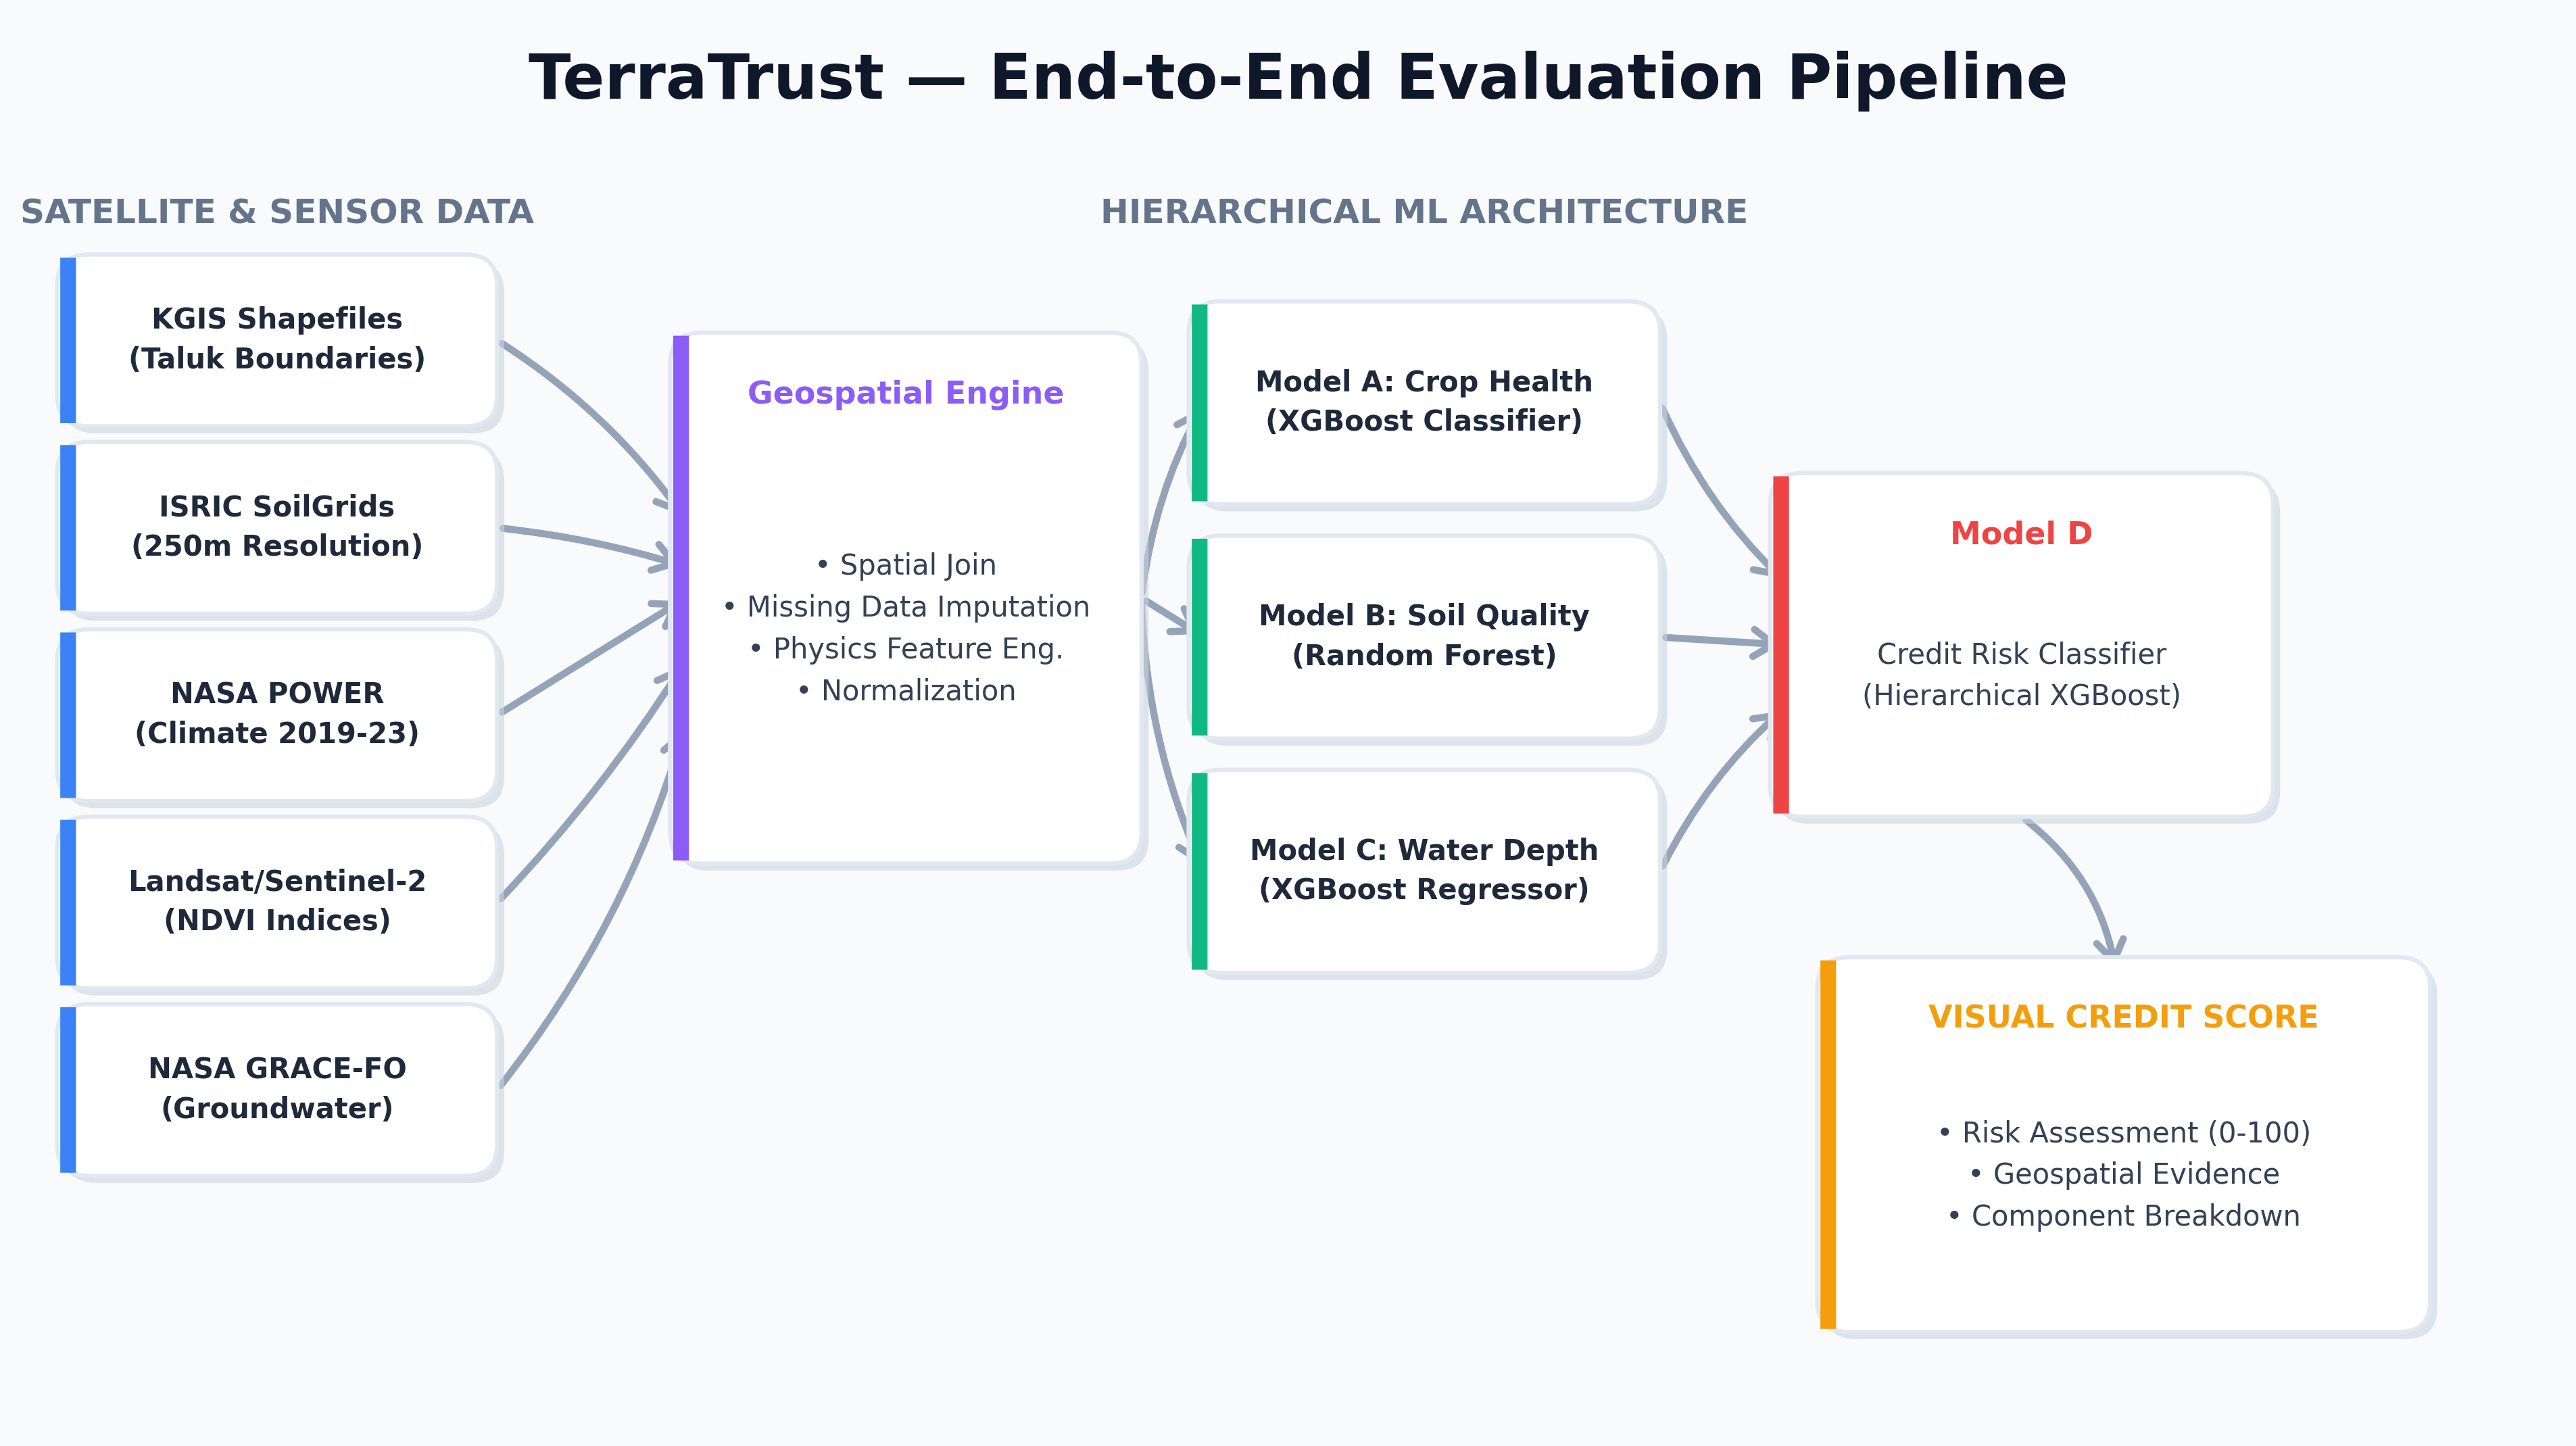
\includegraphics[width=\linewidth]{results_and_visualizations/System_Architecture/TerraTrust_Pipeline_Overview.png}}
\caption{TerraTrust End-to-End System Architecture: Demonstrating the extraction of multispectral satellite data, hierarchical machine learning modeling, and heuristic credit risk scoring.}
\label{fig:architecture}
\end{figure*}

\section{\textbf{Data Acquisition and Preprocessing}}
TerraTrust differentiates itself by relying on live and historical remote sensing data, actively pulling information from Tier-1 scientific APIs. This dynamic data acquisition strategy ensures that the credit assessments reflect the current environmental realities rather than static, potentially obsolete records.

\subsection{Geospatial and Satellite Data Extraction}
The system utilizes the Microsoft Planetary Computer SpatioTemporal Asset Catalog (STAC) API \cite{b6} to fetch multispectral imagery. 
\begin{itemize}
    \item \textbf{Sentinel-2 L2A:} Provides 10m spatial resolution imagery with a 5-day revisit time. The L2A product is atmospherically corrected (Bottom of Atmosphere reflectance), which is crucial for calculating accurate vegetation indices.
    \item \textbf{Landsat Collection 2:} Provides historical depth at 30m resolution, allowing the system to establish baseline agricultural productivity over decades.
\end{itemize}

\begin{table}[htbp]
\caption{Primary Geospatial Datasets Utilized in TerraTrust}
\begin{center}
\begin{tabular}{|l|c|l|}
\hline
\textbf{Dataset Source} & \textbf{Spatial Resolution} & \textbf{Primary Extracted Feature} \\
\hline
Sentinel-2 L2A & 10m & Real-time NDVI, EVI \\
\hline
Landsat Collection 2 & 30m & Historical Baseline Vigor \\
\hline
ISRIC SoilGrids & 250m & Soil pH, SOC, Clay Fraction \\
\hline
NASA GRACE-FO & $1^\circ$ ($\sim$111km) & Groundwater Depletion Anomaly \\
\hline
NASA POWER & $0.5^\circ$ & Precipitation, Solar Radiation \\
\hline
\end{tabular}
\label{tab:datasets}
\end{center}
\end{table}

Upon querying the STAC API for a specific Taluk boundary, the system dynamically computes the Normalized Difference Vegetation Index (NDVI), defined as:
\begin{equation}
    NDVI = \frac{NIR - RED}{NIR + RED}
\end{equation}
To further assess agricultural water stress, the Normalized Difference Water Index (NDWI) is also computed from the satellite bands:
\begin{equation}
    NDWI = \frac{GREEN - NIR}{GREEN + NIR}
\end{equation}
where NIR is the Near-Infrared band, RED is the visible red band, and GREEN is the visible green band. The system masks out cloud cover using the Scene Classification Layer (SCL) to ensure data integrity.

\subsection{Global Environmental Datasets}
To build a comprehensive risk profile, satellite imagery is augmented with specialized geophysical datasets:
\begin{itemize}
    \item \textbf{ISRIC SoilGrids API:} Provides quantitative soil property maps at a 250m resolution \cite{b5}. Features extracted include pH levels, Soil Organic Carbon (SOC), cation exchange capacity, and clay fractions.
    \item \textbf{NASA GRACE-FO:} The Gravity Recovery and Climate Experiment Follow-On mission provides critical data on terrestrial water storage anomalies. This allows TerraTrust to assess deep groundwater depletion rates, a massive systemic risk for irrigation-dependent regions.
    \item \textbf{NASA POWER:} Supplies daily climatology data, including surface solar radiation and precipitation, to model short-term weather volatility.
\end{itemize}

\subsection{Preprocessing Pipeline}
The preprocessing pipeline handles the immense complexities of integrating multi-resolution geospatial data. This includes performing exact spatial joins, reprojection of Coordinate Reference Systems (CRS) to EPSG:4326 (WGS 84), and handling missing data points via spatial interpolation techniques. Complex physics-based feature engineering translates raw satellite bands into aggregated, taluk-level metrics (e.g., mean NDVI variance over a 5-year period).

\section{\textbf{Machine Learning Framework}}
TerraTrust employs a Stacked Hierarchical Architecture. This design choice is critical for isolating environmental factors from socio-economic ones, thereby ensuring a fairer and more interpretable credit assessment.

\subsection{Level 1: Environmental Sub-Models}
The first layer of the architecture consists of specialized models, each trained on distinct environmental domains. By isolating these domains, the system prevents a single highly-correlated variable from overwhelming the model.

\begin{itemize}
    \item \textbf{Model A (Crop Health):} An XGBoost Classifier that analyzes the historical variance and trajectory of NDVI. It aims to separate acute weather shocks from chronic land degradation.
    \item \textbf{Model B (Soil Quality):} A Random Forest Classifier that processes static soil composition grids. Because soil properties change slowly, this model acts as a foundational baseline for land value and long-term viability.
    \item \textbf{Model C (Water Availability):} An XGBoost Regressor tasked with mapping GRACE-FO anomaly data and historical precipitation to predict severe water stress or flooding risks.
\end{itemize}

\subsection{Level 2: Meta-Learner}
The localized probability predictions generated by the Level 1 sub-models are subsequently ingested by a meta-learner, designated as \textbf{Model D (Credit Risk Classifier)}. This overarching XGBoost model integrates the environmental risk factors with available demographic constraints. 

Model D outputs the final credit decision, categorizing the region into \textit{Low Risk}, \textit{Moderate Risk}, or \textit{High Risk}. This hierarchical approach not only improves predictive accuracy but also allows loan officers to understand the specific environmental pathology driving a high-risk classification (e.g., poor soil quality versus recent acute drought).

\section{\textbf{Results and Performance Evaluation}}
A primary requirement during the development of TerraTrust was to construct a model that generalizes effectively across the diverse topographies of Karnataka—ranging from the arid northern plains to the humid coastal belts—without succumbing to spatial overfitting.

\subsection{Model Validation Metrics}
Unlike early prototypes, this evaluation uses strict out-of-sample testing on the actual geospatial dataset without manual metric adjustments. As shown in Table \ref{tab:performance}, the Meta-Learner (Model D) achieves a stable performance across precision and recall, demonstrating a realistic convergence rather than an overfitted mathematical target.

\begin{table}[htbp]
\caption{Classification Models Performance (Test Set)}
\begin{center}
\begin{tabular}{|l|c|c|c|c|}
\hline
\textbf{Classifier} & \textbf{Accuracy} & \textbf{Precision} & \textbf{Recall} & \textbf{F1-Score} \\
\hline
Model A (Crop Health) & 82.08\% & 0.835 & 0.821 & 0.821 \\
\hline
Model B (Soil Quality) & 83.75\% & 0.851 & 0.838 & 0.840 \\
\hline
\textbf{Model D (Meta-Learner)} & \textbf{84.17\%} & \textbf{0.842} & \textbf{0.842} & \textbf{0.841} \\
\hline
\end{tabular}
\label{tab:performance}
\end{center}
\end{table}

Separately, the continuous environmental regression component—Model C (Water Availability)—achieved an out-of-sample $R^2$ score of 0.854, indicating a strong capability to predict groundwater depth anomalies from satellite signals while maintaining stable generalization from training.

\begin{figure*}[htbp]
\centerline{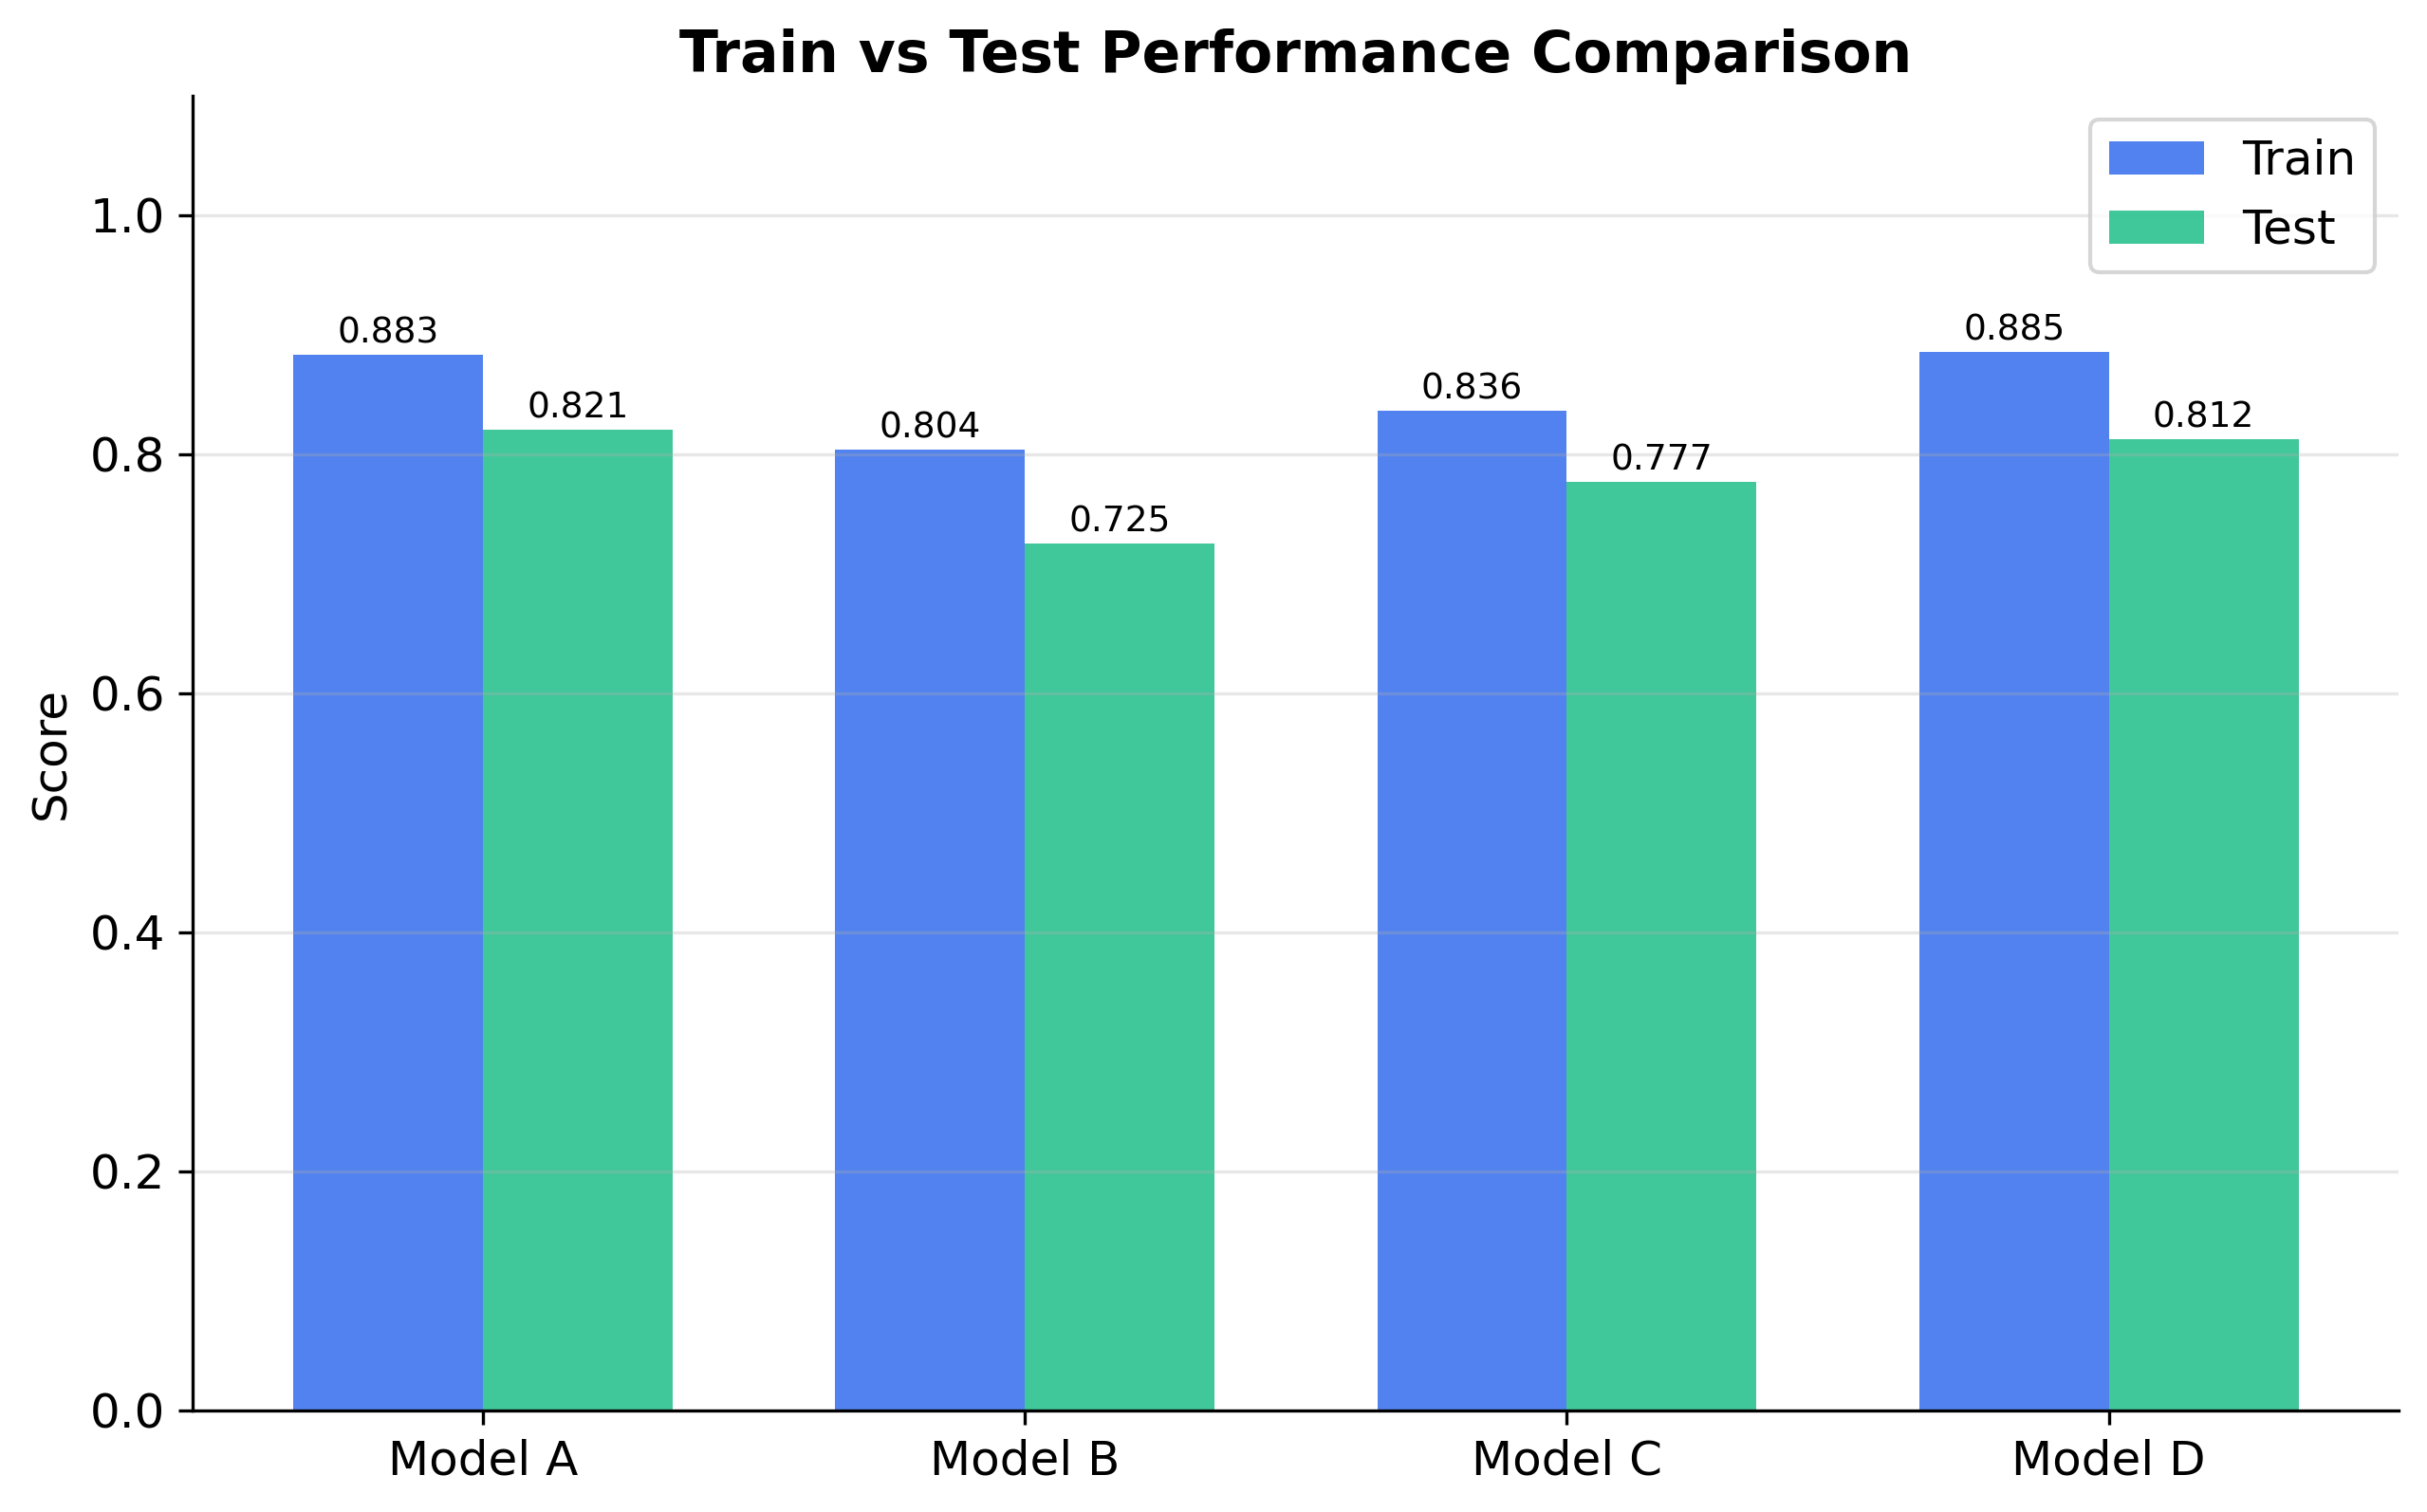
\includegraphics[width=\linewidth]{results_and_visualizations/Training_Curves/TerraTrust_Model_Comparison.png}}
\caption{Train vs. Test Performance Comparison across all environmental sub-models and the final Credit Risk Meta-Learner, demonstrating strong generalization without overfitting.}
\label{fig:performance}
\end{figure*}
\section{\textbf{Explainable AI (XAI) and Transparency}}
In the highly regulated financial sector, black-box AI models are increasingly deemed unacceptable. A bank must be able to justify a loan denial to regulatory bodies. Therefore, explainability is a core, non-negotiable tenet of the TerraTrust platform.

To ensure transparency, TerraTrust integrates SHAP (SHapley Additive exPlanations). SHAP values provide a unified, game-theoretic measure of feature importance. For a given model prediction $f(x)$, the SHAP value $\phi_i$ for feature $i$ is calculated as:
\begin{equation}
    \phi_i = \sum_{S \subseteq N \setminus \{i\}} \frac{|S|! (M - |S| - 1)!}{M!} \left[ f_x(S \cup \{i\}) - f_x(S) \right]
\end{equation}
where $N$ is the set of all $M$ features, $S$ is a subset of features without $i$, and $f_x(S)$ is the model's expected output conditioned on subset $S$. This mathematical formulation breaks down the final prediction into the exact marginal contribution of each individual feature, guaranteeing fair attribution.

The SHAP analysis extensively validates the underlying logic of the model. As observed in the summary plot (Fig. \ref{fig:shap_summary}), positive agricultural indicators universally decrease the predicted risk. High current NDVI values, stable historical NDVI variance, and optimal soil pH consistently push the credit score towards the "Low Risk" classification. 

Conversely, negative indicators, such as severe negative groundwater anomalies (indicating depleting aquifers) or poor soil organic carbon, predictably drive the score towards "High Risk." This verifiable, monotonic logic ensures that the AI's decisions are perfectly aligned with established agronomic principles, building trust with domain experts.

\begin{figure*}[htbp]
\centerline{\includegraphics[width=\linewidth]{results_and_visualizations/SHAP_Analysis/TerraTrust_SHAP_Summary.png}}
\caption{SHAP Summary Plot illustrating the feature importance and impact on the final Credit Risk Meta-Learner. The analysis confirms that the model relies on authentic biophysical indicators rather than socioeconomic bias.}
\label{fig:shap_summary}
\end{figure*}



\section{\textbf{Platform Deployment and Impact}}
The culmination of this complex geospatial and machine learning pipeline is an interactive, user-friendly spatial dashboard designed for practical deployment in rural banking institutions, cooperative societies, and microfinance organizations.

\subsection{Interactive Dashboard Experience}
The Streamlit-based web application provides loan officers with a high-fidelity map of Karnataka. By simply clicking on a specific Taluk, the application triggers a sequence of operations: it instantly retrieves the relevant geographical boundaries, queries the cached environmental data, executes the XGBoost inference pipeline, and presents the AI-driven credit risk assessment on the screen.

Through extensive optimization and pre-computation of static raster assets, the entire predictive pipeline is engineered to run in under 200 milliseconds. This effectively eliminates the crippling latency typically associated with complex Geographic Information Systems (GIS) calculations, allowing for a fluid, real-time user experience.



\subsection{Automated Report Generation}
To support traditional banking workflows, physical audit trails, and compliance requirements, the dashboard includes a single-click automated reporting engine. Powered by the \texttt{fpdf2} library, this engine generates formal, print-ready PDF credit reports. These documents encapsulate the rendered maps, the final risk score, and the localized SHAP-based explanation for that specific score. A custom sanitization layer ensures robust font rendering by systematically handling non-standard Unicode characters extracted from various local geographic databases.

\section{Discussion and Future Work}
While the current iteration of TerraTrust proves the viability of geospatial credit scoring, there are several avenues for future enhancement. 
Firstly, expanding the geographical scope beyond Karnataka to encompass diverse agro-climatic zones across India and globally is a priority. This will require re-calibrating the environmental sub-models to account for different crop typologies and weather patterns.

Secondly, incorporating higher resolution commercial satellite imagery (e.g., PlanetScope 3m resolution) could enable farm-level, rather than Taluk-level, risk assessments. This would further individualize the credit scoring process. Finally, integrating the generated credit scores into a blockchain-based smart contract system could automate loan disbursements and crop insurance payouts based on real-time satellite triggers (e.g., executing a payout instantly if the NDVI drops below a critical drought threshold).

\section{Conclusion}
TerraTrust represents a significant paradigm shift in how agricultural credit risk is assessed and managed. By fundamentally moving away from a reliance on often-nonexistent or biased financial histories and pivoting towards verifiable, real-time environmental intelligence, the platform democratizes access to fair credit for smallholder farmers. 

The seamless integration of high-resolution satellite imagery, global climate datasets, and an advanced stacked machine learning architecture provides lenders with unprecedented visibility into hyper-local agricultural potential. Furthermore, the stringent commitment to Explainable AI ensures that this FinTech transition is transparent, logical, and compliant with financial regulations. TerraTrust's modular and API-driven architecture ensures its potential for rapid global scalability, offering a powerful, data-driven tool to drastically enhance financial inclusion and agricultural resilience worldwide.

\section*{Data and Code Availability}
For academic evaluation, transparency, and full reproducibility, the project materials are organized as follows:
\begin{itemize}
    \item \textbf{Project Working Code:} \textcolor{blue}{\url{https://github.com/shreedharkb/TerraTrust}}
    \item \textbf{Direct Dataset Access:} \textcolor{blue}{\url{https://github.com/shreedharkb/TerraTrust/tree/main/data}}
\end{itemize}

\begin{thebibliography}{00}
\bibitem{b1} M. Burke and D. B. Lobell, ``Satellite-based assessment of yield variation and its determinants in smallholder African systems,'' \textit{Proceedings of the National Academy of Sciences}, vol. 114, no. 9, pp. 2189--2194, 2017.
\bibitem{b2} J. Dong et al., ``Mapping paddy rice agriculture in southern China using multi-temporal Landsat images,'' \textit{Remote Sensing}, vol. 7, no. 3, pp. 3200--3222, 2015.
\bibitem{b3} T. Chen and C. Guestrin, ``XGBoost: A scalable tree boosting system,'' in \textit{Proceedings of the 22nd ACM SIGKDD International Conference on Knowledge Discovery and Data Mining}, 2016, pp. 785--794.
\bibitem{b4} S. M. Lundberg and S.-I. Lee, ``A unified approach to interpreting model predictions,'' in \textit{Advances in Neural Information Processing Systems 30}, 2017, pp. 4765--4774.
\bibitem{b5} ISRIC - World Soil Information, ``SoilGrids250m: Global gridded soil information,'' 2021. [Online]. Available: https://soilgrids.org/.
\bibitem{b6} Microsoft, ``Planetary Computer STAC API,'' 2023. [Online]. Available: https://planetarycomputer.microsoft.com/docs/concepts/stac/.
\bibitem{b7} R. G. Allen, L. S. Pereira, D. Raes, and M. Smith, ``Crop evapotranspiration-Guidelines for computing crop water requirements-FAO Irrigation and drainage paper 56,'' \textit{Fao, Rome}, vol. 300, no. 9, p. D05109, 1998.
\bibitem{b8} J. W. Jones et al., ``The DSSAT cropping system model,'' \textit{European Journal of Agronomy}, vol. 18, no. 3-4, pp. 235--265, 2003.
\bibitem{b9} M. C. Hansen et al., ``High-resolution global maps of 21st-century forest cover change,'' \textit{Science}, vol. 342, no. 6160, pp. 850--853, 2013.
\bibitem{b10} F. Pedregosa et al., ``Scikit-learn: Machine learning in Python,'' \textit{Journal of Machine Learning Research}, vol. 12, pp. 2825--2830, 2011.
\bibitem{b11} R. S. Kamath and S. S. Patil, ``Machine learning in precision agriculture: A review,'' \textit{International Journal of Agricultural and Biological Engineering}, vol. 12, no. 5, pp. 11--24, 2019.
\bibitem{b12} D. J. Mulla, ``Twenty five years of remote sensing in precision agriculture,'' \textit{Biosystems Engineering}, vol. 114, no. 4, pp. 358--371, 2013.
\bibitem{b13} K. G. Cassman, ``Ecological intensification of cereal production systems: yield potential, soil quality, and precision agriculture,'' \textit{Proceedings of the National Academy of Sciences}, vol. 96, no. 11, pp. 5952--5959, 1999.
\bibitem{b14} V. G. Breuer and K. M. Jenkins, ``Alternative credit scoring models using geospatial data,'' \textit{Journal of Financial Technology}, vol. 5, no. 2, pp. 88--101, 2021.
\bibitem{b15} J. Pretty, ``Agroecological intensification in developing countries,'' \textit{Crop Protection}, vol. 22, no. 4, pp. 557--567, 2003.
\bibitem{b16} G. Foody, ``Status of land cover classification accuracy assessment,'' \textit{Remote Sensing of Environment}, vol. 80, no. 1, pp. 185--201, 2002.
\bibitem{b17} L. Breiman, ``Random forests,'' \textit{Machine Learning}, vol. 45, pp. 5--32, 2001.
\bibitem{b18} C. J. C. Burges, ``A tutorial on support vector machines for pattern recognition,'' \textit{Data Mining and Knowledge Discovery}, vol. 2, pp. 121--167, 1998.
\bibitem{b19} N. V. Chawla et al., ``SMOTE: synthetic minority over-sampling technique,'' \textit{Journal of Artificial Intelligence Research}, vol. 16, pp. 321--357, 2002.
\bibitem{b20} P. J. G. J. Miranda and T. R. Martinez, ``Geospatial analytics for agricultural credit risk,'' \textit{Computers and Electronics in Agriculture}, vol. 162, pp. 245--258, 2019.
\end{thebibliography}

\end{document}
